\documentclass[12pt]{article}
\usepackage[left=1in,right=1in,top=0.75in,bottom=1in]{geometry} % never use the anysize package!
\usepackage{tabularx}
\usepackage{xcolor}
\usepackage{tikz}
\usepackage[american, EFvoltages, cuteinductors]{circuitikz}

\fboxsep = 6.0pt
\parskip = 6.0pt
\parindent = 0.0pt
\hfuzz = 18.0pt

\graphicspath{{../images/}{../soldering/}}
% tikz stuff and other macros
% Jesse Hamner
% 2013--2024

\usepackage{tabularx}

\newcolumntype{R}[2]{%
    >{\adjustbox{angle=#1,lap=\width-(#2)}\bgroup}%
    l%
    <{\egroup}%
}


% make a few color defs:
\definecolor{rltbrightred}{rgb}{1,0,0}
\definecolor{rltred}{rgb}{0.75,0,0}
\definecolor{rltdarkred}{rgb}{0.5,0,0}
\definecolor{rltbrightgreen}{rgb}{0,0.75,0}
\definecolor{rltgreen}{rgb}{0,0.5,0}
\definecolor{rltdarkgreen}{rgb}{0,0.25,0}
\definecolor{rltbrightblue}{rgb}{0,0,1}
\definecolor{rltblue}{rgb}{0,0,0.75}
\definecolor{rltdarkblue}{rgb}{0,0,0.5}
%\definecolor{webred}{rgb}{0.5,.25,0}
\definecolor{webblue}{rgb}{0,0,0.75}
\definecolor{webgreen}{rgb}{0,0.5,0}
\definecolor{lightgray}{gray}{0.9}
\definecolor{medgray}{gray}{0.6}
\definecolor{footlineblue}{rgb}{0.392,0.706,0.941}
\definecolor{darkgreen}{rgb}{0.00,0.50,0.00}
\definecolor{gray50}{gray}{0.50}
\definecolor{gray95}{gray}{0.95}
\definecolor{webred}{rgb}{0.75,0,0.0}

\renewcommand{\thefootnote}{\fnsymbol{footnote}}
\newcommand{\sep}{1mm}
\newcommand{\negsep}{-4mm}
\newcommand{\widesep}{7mm}
\newcommand{\thisscale}{0.6}
\newcommand{\grr}{\rowcolor{gray!15}}

\newcommand{\+}{\item}		% easier than typing \item a lot
\newcommand{\bi}{\begin{itemize}}
\newcommand{\ei}{\end{itemize}}
\newcommand{\bd}{\begin{description}}
\newcommand{\ed}{\end{description}}
\newcommand{\be}{\begin{enumerate}}
\newcommand{\ee}{\end{enumerate}}
\newcommand{\rr}{\raggedright}

\newcommand{\cb}{\cellcolor{black!35}}

\newcommand{\ckb}{\item[$\square$]} % list checkboxes (requires marvosym)

% A command that makes a uniform box around a paragraph. 
% It's a minipage environment, which means it doesn't support some commands.
\newcommand{\stbox}[2]{
	\begin{center}
	\fbox{
		\begin{minipage}[c]{#1}{
		\noindent #2
		}
		\end{minipage}
	}
	\end{center}
}


% A series of macros that enable programmatic of drawing stylized
% ions, protons, or electrons.
% Supports,  e.g., richer drawings of capacitors or
% current flowing in wires:

\newcommand{\ionradius}{0.06} % TODO should make it possible to change this too

\newcommand{\drawion}[4]{
		\draw [black, very thin] (#1,#2) circle [radius=#3];
		\node[scale=0.3, thick ] at (#1,#2) {#4};
}

\newcommand{\posion}[3]{
		\drawion{#1}{#2}{#3}{$+$}
		}

\newcommand{\negion}[3]{
		\drawion{#1}{#2}{#3}{$-$}
		}

\newcommand{\horizionarray}[4]{
	\newdimen\len
	\len=#1 cm
	\advance\len by -0.4cm
	\drawion{\len}{#2}{\ionradius}{#4}
	\advance\len by 0.15cm
	\drawion{\len}{#2}{\ionradius}{#4}
	\advance\len by 0.15cm
	\drawion{\len}{#2}{\ionradius}{#4}
	\advance\len by 0.2cm
	\drawion{\len}{#2}{\ionradius}{#4}
	\advance\len by 0.15cm
	\drawion{\len}{#2}{\ionradius}{#4}
	\advance\len by 0.15cm
	\drawion{\len}{#2}{\ionradius}{#4}
}

\newcommand{\vertionarray}[4]{
	\newdimen\len
	\len=#2 cm
	\advance\len by -0.4cm
	\drawion{#1}{\len}{\ionradius}{#4}
	\advance\len by 0.15cm
	\drawion{#1}{\len}{\ionradius}{#4}
	\advance\len by 0.15cm
	\drawion{#1}{\len}{\ionradius}{#4}
	\advance\len by 0.2cm
	\drawion{#1}{\len}{\ionradius}{#4}
	\advance\len by 0.15cm
	\drawion{#1}{\len}{\ionradius}{#4}
	\advance\len by 0.15cm
	\drawion{#1}{\len}{\ionradius}{#4}
}



% Nokia 84 x 48 pixel LCD screen (usually model number 5110 or 3310)
\newcommand{\drawnokiagrid}{
\draw[step=1cm,blue!30,very thin] (0,0) grid (6,8);
\foreach \x in {0,1,2,3,4,5}
	\draw (\x cm, 0pt) -- (\x cm, -3pt) node[anchor=north] {$\x$};
\foreach \y in {1,2,3,4,5,6,7,8}
	\draw (0pt, \y cm) -- (-3pt, \y cm) node[anchor=east] {$\y$};
}


% part of the Nokia grid set of commands
\newcommand{\msqo}[3]{
\def\mycmd{#3}

\if\mycmd1
	\msq{#1}{#2}{black!65}
\else
	\msq{#1}{#2}{white}
\fi
}


% part of the Nokia grid set of commands
\newcommand{\msq}[3]{
\edef\myx{#1}
\pgfmathparse{\myx+1.0}
\edef\myxtwo{\pgfmathresult}
\edef\myy{#2}
\pgfmathparse{\myy+1.0}
\edef\myytwo{\pgfmathresult}
\fill[#3] (\myx,#2) rectangle (\myxtwo,\myytwo);}


% part of the Nokia grid set of commands
\newcommand{\mcol}[9]{
\msqo{#1}{#2}{#3}
\msqo{#1}{#4}{#5}
\msqo{#1}{#6}{#7}
\msqo{#1}{#8}{#9}
}


% part of the Nokia grid set of commands
\newcommand{\hexlabel}[5]{
\node[rotate=90] at (0.5,-1) {\Large\texttt{#1}};
\node[rotate=90] at (1.5,-1) {\Large\texttt{#2}};
\node[rotate=90] at (2.5,-1) {\Large\texttt{#3}};
\node[rotate=90] at (3.5,-1) {\Large\texttt{#4}};
\node[rotate=90] at (4.5,-1) {\Large\texttt{#5}};
}



% drawing cubes using TikZ:
\newcommand{\makecube}[2]{
\begin{tikzpicture}[xscale=#2,yscale=#2]
\foreach \x in{0,...,#1}
{   \draw (0,\x ,#1) -- (#1,\x ,#1);
    \draw (\x ,0,#1) -- (\x ,#1,#1);
    \draw (#1,\x ,#1) -- (#1,\x ,0);
    \draw (\x ,#1,#1) -- (\x ,#1,0);
    \draw (#1,0,\x ) -- (#1,#1,\x );
    \draw (0,#1,\x ) -- (#1,#1,\x );
}
\end{tikzpicture}
}


% Draw faux-3D squares or cubes:
\newcommand{\makeplate}[3]{
\begin{tikzpicture}[xscale=#3,yscale=#3]

\foreach \x in {0,...,#1}
{
	\filldraw[gray95, fill=gray95, line width=0.0cm] (0,#1,0) -- (0,#1,#2) -- (#1,#1,#2) -- (#1,#1, 0) -- (0,#1,0) -- cycle;
	\filldraw[gray50, fill=gray50, line width=0.0cm] (#1,#1,0) -- (#1,#1,#2) -- (#1,0,#2) -- (#1,0, 0) -- (#1,#1,0) -- cycle;
}

\foreach \x in{0,...,#1}
{   \draw (0,\x ,#2) -- (#1,\x ,#2);
    \draw (\x ,0,#2) -- (\x ,#1,#2);
	\draw (#1,\x ,#2 ) -- (#1,\x ,0);
    \draw (\x ,#1,#2 ) -- (\x ,#1,0);
}

\foreach \x in {0,...,#2}
{
    \draw(#1,0,\x  ) -- (#1,#1,\x );
    \draw(0,#1,\x  ) -- (#1,#1,\x );
}

\foreach \x in{1,...,#1}
{
\node[align=left] at (\x-0.5,#1-0.5,#2) {\x};
}

\foreach \x in{#1,...,2}
{
\node[align=left] at (0.5,#1-\x+0.5,#2) {\x};
}

%\draw[webred, thick](0,0,0) -- (0,0,#2);
%\draw[webblue, thick](0,0,0) -- (#1,0,0);
%\draw[darkgreen, thick](0,0,0) -- (0,#1,0);

\end{tikzpicture}
}


% Draw a line of faux-3D shaded blocks using TikZ:
\newcommand{\blockline}[2]{
\begin{tikzpicture}[xscale=#2,yscale=#2]

\filldraw[fill=gray95, ultra thin] (0,1,0) -- (0,1,1) -- (#1,1,1) -- (#1,1, 0) -- (0,1,0) -- cycle;
\filldraw[fill=gray50, ultra thin] (#1,1,0) -- (#1,1,1) -- (#1,0,1) -- (#1,0, 0) -- (#1,1,0) -- cycle;

\draw (0,1,0 ) -- (#1,1,0); % top line
\draw (#1,1,1) -- (#1,1,0);
\draw (#1,0,1) -- (#1,1,1);
\draw (0,1, 1) -- (#1,1,1);
\draw (0,0,1 ) -- (#1,0,1);

\foreach \x in{0,...,#1}
{   
    \draw (\x ,0,1) -- (\x ,1,1 ); % straight vertical lines    
    \draw (\x ,1,1) -- (\x ,1,0 );
}

\foreach \x in{1,...,#1}
{
	\node[align=left] at (\x-0.5,0.5,1) {\x};
}

\end{tikzpicture}
}


% make a blank line under which, e.g., someone could write an unknown answer:
\newcommand{\makeblank}[1]{
\underline{\makebox[#1][l]{}}
}


% tilt the text atop a table row at an angle:
\newcommand*\rot{\multicolumn{1}{R{55}{1.2ex}}}% no optional argument here, please!


\newcommand{\adderblock}[3]{

	\begin{scope}

	\draw (0,#1)
	  [xshift = 2.5cm]
	  node[one bit adder, scale=0.75](fa#2){}
	  node[xshift=0.75cm, yshift=1cm](fa#2carrylabel){\footnotesize $Carry_#3$}
  	  node[ocirc, xshift=1.5cm, label={[label distance=0mm]0:$Sum_#3$}](fa#2sum){}
	;

    \draw (0.5,#1)
 	  [yshift=-0.65cm] 
	  node[american xor port](axorb#2){}
	  node[ocirc, xshift = -2.2cm, yshift = -0.28cm](axorb#2node){}
   	  node[xshift = -2.6cm, yshift = 0mm](){{\color{red}$A_{#3}$}}
	  node[xshift = 0.2cm, yshift = 6mm] {{\footnotesize{$XOR_{#3}$}}}
   	  node[ocirc, xshift = -4.5cm, yshift = 0.32cm](m#2node){}
	  node[xshift = -4.0cm, yshift = 0.6cm, color=rltred]{\color{rltred}$M_{#3}$}
	;
 
    \draw (0,#1)
	  [yshift=0.65cm]
	  node[ocirc, xshift = -2.0cm](b#2node){}
   	  node[xshift = -2.3cm, yshift = 3mm](){{\color{blue}$B_{#3}$}}
    ;
  
    \draw (0,#1)
	  [color=blue] 
	  (b#2node) -- (fa#2.lpin 1) 
	;
  
    \draw
	  [color=rltred] 
	  (m#2node) -- (axorb#2.in 1) 
	;

    \draw (0,#1)
	  (axorb#2node) -- (axorb#2.in 2)
	  (fa#2.rpin 1) -- (fa#2sum)
	;
	
    \draw(0, #1)[color=brown, very thick]
      (axorb#2.out) -- (fa#2.lpin 2)
    ;
    
  \end{scope}
}



% Half Adder Symbol:
\newcommand{\halfadder}{
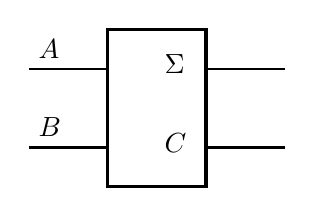
\begin{tikzpicture}

\draw [very thick] (0,0) -- (1.25,0) -- (1.25,2) -- (0,2) -- cycle;
\draw [thick] (-1,0.5) -- (0,0.5);
\draw [thick] (-1,1.5) -- (0,1.5);
\draw [thick] (1.25,0.5) -- (2.25,0.5);
\draw [thick] (1.25,1.5) -- (2.25,1.5);

\node[xshift=-10mm, yshift=20mm, anchor= north west] {$A$};
\node[xshift=-10mm, yshift=10mm, anchor= north west] {$B$};
\node[xshift=6mm, yshift=18mm, anchor= north west] {$\Sigma$};
\node[xshift=6mm, yshift=8mm, anchor= north west] {$C$};

\end{tikzpicture}
}


% Full Adder Symbol:
\newcommand{\fulladder}{
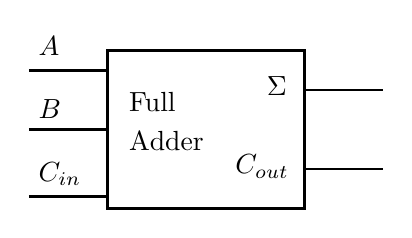
\begin{tikzpicture}

\draw [very thick] (0,0) -- (2.5,0) -- (2.5,2) -- (0,2) -- cycle;
\draw [thick] (-1,0.15) -- (0,0.15);
\draw [thick] (-1,1.0) -- (0,1.0);
\draw [thick] (-1,1.75) -- (0,1.75);

\draw [thick] (2.5,0.5) -- (3.5,0.5);
\draw [thick] (2.5,1.5) -- (3.5,1.5);

\node[xshift=-10mm, yshift=23mm, anchor= north west] {$A$};
\node[xshift=-10mm, yshift=15mm, anchor= north west] {$B$};
\node[xshift=-10mm, yshift=7mm, anchor= north west] {$C_{in}$};

\node[xshift=19mm, yshift=18mm, anchor= north west] {$\Sigma$};
\node[xshift=15mm, yshift=8mm, anchor= north west] {$C_{out}$};
\node[xshift=1.5mm, yshift=16mm, anchor= north west] {Full};
\node[xshift=1.5mm, yshift=11mm, anchor= north west] {Adder};

\end{tikzpicture}
}


\begin{document}

\title{Logic Gate Puzzles}
\author{A Fun Resource for the Computing Workshop}
\date{}
\maketitle



\section*{Introduction}

This section contains some logic puzzles that help you cement your understanding of how using gates together can check inputs and provide outputs according to the questions you specify. The challenges start with simple examples and move to more challenging questions. Every puzzle has an answer provided in the answer key.

Each puzzle's objective is to solve the question asked, using as few gates as possible. There are many possible solutions, but the solutions focus on one straightforward answer, and sometimes a more clever answer where it exists. All puzzles have similar rules.

\begin{itemize}
\item The solution must only use OR gates, AND gates, and NOT gates
\item There must be a single output to check for the result (that is, you can't ask the user to check three separate AND gates to see if $AB$, $AC$, or $BC$ are ``true'')
\end{itemize}

Some other parameters:
\begin{itemize}
\item You can connect signals to more than one gate at a time if you want to
\item You can connect inputs to each other if it helps
\item You may not have to build a circuit to handle every case
\end{itemize}

Your first move should be to understand the potential combinations of inputs and how to test them. Don't think about testing all of them at once. Start small. There may not be more than one thing to test, but if you need to, figure out the smallest test that helps you out, and then move on to the next one. You may have to figure out how the results of some tests must be compared: you may need to add AND, NOT, and OR comparisons to some of the results of individual tests.


\newpage

\subsection*{Puzzle 1}

Which circuit will create the following truth table?

\begin{tabular}{ll | c}
\multicolumn{3}{c}{\textbf{Truth Table}}\\
\hline\\[\negsep]
\textbf{A} & \textbf{B} & \textbf{OUT}\\
\hline
0 & 0 & 0  \\
1 & 0 & 1  \\
0 & 1 & 1  \\
1 & 1 & 1  \\
\hline
\end{tabular}



\clearpage
\newpage

\subsection*{Puzzle 2}

Design a circuit that tests to see if A is TRUE (has an output of 1) and B is FALSE (has an output of 0). You do not need to check to see if A is FALSE and B is TRUE.



\clearpage
\newpage

\subsection*{Puzzle 3}

Design a circuit that tests to see if A is \emph{different from} B, no matter what value A has. \emph{Hint: the solution to Puzzle 1 is a huge chunk of the answer.}



\clearpage
\newpage

\subsection*{Puzzle 4}

Say you had three inputs $A$, $B$, and $C$, and you want to know when a majority of them are ON or TRUE.
The question is simple enough: with three inputs, use connected logic gates in a way that can tell when the majority of inputs (here, that's at least two of the three) have a 1 as their input value.

\subsubsection*{Setting Up}

Start by taking a minute to think of the way to test if some pair of inputs are both 1. We will need to test each possible pair of inputs. That may seem like a big deal, but we can break it down into small chunks.

There's a way to represent all of the possible conditions in a compact way.
Let's start by saying a line over the letter indicates ``NOT true'', and no line over the letter indicates ``true''.
\begin{itemize}
\item If all of the inputs are off, then the condition can be represented by: $\overline{ABC}$. 
\item When all inputs are on, the shorthand would be $ABC$. 
\item When only A is off, the condition is represented by $\overline{A}BC$. 
\end{itemize}

We must first find any combination of the three signals that has two or more of them reporting ``yes''. Then we can determine how we might test the signals. How might you break up the problem into tests of two inputs? 

Returning to our setup: how many combinations are there in total?

\begin{enumerate}
\item Each input can be 1 or 0 -- there are exactly two possible states
\item There are three inputs in total, and each can be on or off
\item Each input is not affected by any other input (the inputs are not tied together in any way)
\end{enumerate}

We need a truth table!
The truth table will have $2 \times 2 \times 2$ (that is, $2^3$) possible combinations. 
So let's make a table by counting from 0 to 7 in binary.
We will assign one of the A, B, or C inputs to each column ($2^0$, $2^1$, and $2^2$).

\renewcommand{\arraystretch}{1.2}

\begin{tabular}{m{2in} m{3in}}

\begin{tabular}{cccc}
\hline
A & B & C & Symbol\\
\hline
0 & 0 & 0 & $\overline{ABC}$\\
0 & 0 & 1 & $\overline{AB}C$\\
0 & 1 & 0 & $\overline{A}B\overline{C}$\\
0 & 1 & 1 & $\overline{A}BC$\\
1 & 0 & 0 & $A\overline{BC}$\\
1 & 0 & 1 & $A\overline{B}C$\\
1 & 1 & 0 & $AB\overline{C}$\\
1 & 1 & 1 & $ABC$\\
\hline
\end{tabular}

&

To cover every possible case, half of of each column will be ``true'' and half will be ``false''.
For the left-most column (``A''), the first four column values are 0 and the next four are 1.
The right-most column alternates ``on-off'' four times, and the middle column alternates off and on every other row.
It looks like we are counting in binary from 0 to 7, because we are! That way we will know we have covered every possible condition that we have to test.

\\
\end{tabular}

\renewcommand{\arraystretch}{1.0}

The table shows us all possible conditions for these three inputs. Now add a results column, showing the answer our logic circuit should produce. Remember, if any two inputs in the row are true, then the result column will be true. Otherwise, the result is false.

\begin{tabular}{m{2in} m{3in}}
\renewcommand{\arraystretch}{1.2}
\begin{tabular}{ccccc}
\hline
A & B & C & Symbol           & Result\\
\hline
0 & 0 & 0 & $\overline{ABC}$ & 0\\
0 & 0 & 1 & $\overline{AB}C$ & 0\\
0 & 1 & 0 & $\overline{A}B\overline{C}$ & 0\\
0 & 1 & 1 & $\overline{A}BC$ & 1\\
1 & 0 & 0 & $A\overline{BC}$ & 0\\
1 & 0 & 1 & $A\overline{B}C$ & 1\\
1 & 1 & 0 & $AB\overline{C}$ & 1\\
1 & 1 & 1 & $ABC$ & 1\\
\hline
\end{tabular}

&

The fourth, sixth, seventh, and eighth rows all have two or more inputs set to ``on''. The results (``R'') column is 1/``true'' for these four rows, and 0/``false'' for the rest. 

\\
\end{tabular}
\renewcommand{\arraystretch}{1.0}

The logic can be expressed like this: 

($A$ AND $B$) OR ($A$ AND $C$) OR ($B$ AND $C$) OR ($A$ AND $B$ AND $C$).

So if any of these individual conditions is true, the result is true.
Note that all three values do not have to be true for the result to be true. Any two true inputs gives the same result as all three inputs being on. So there is no need to specifically test for all three inputs being true.




\end{document}
